\chapter{Integrating Fetch and Decode}

\section{Integration}
We now have working Fetch, Decode, and Execute modules.  Now it is time to put them together to produce a system that can:
\begin{enumerate}
	\item Update the program counter
	\item Read the appropriate instruction from the instruction datafile
	\item Read the correct registers
	\item Update all control lines
	\item Sign extend address data
	\item Calculate Branch Target Addresses
	\item Provide a zero bit for conditional branch instructions
	\item Produce ALU results for R-Type and D-Type instructions
\end{enumerate}

Once we can do all of this, we will be ready for the iMemory stage.  We currently have the fetch and decode module integrated into datapath.v.  We also have a working execute module.  Today we need to integrate the Execute module into datapath.v.  Please reuse the instructions from your Expected Results Table that you used when you integrated fetch and decode.  Please make sure that datapath.v is the "top module" in your project.  Once integrated, you should be able to produce a simulation that includes 3 new outputs:
\begin{enumerate}
	\item Branch Target
	\item ALU Result
	\item Zero
\end{enumerate}   

These three new outputs are marked on Figure Figure ~\ref{fig:integrated_execute}.  To verify these outputs, you should update the Expected Results Table to include these three outputs.  Then you should verify this table against your simulation results.

\begin{figure}
	\caption{Execute Stage}\label{fig:integrated_execute}
	\begin{center}
		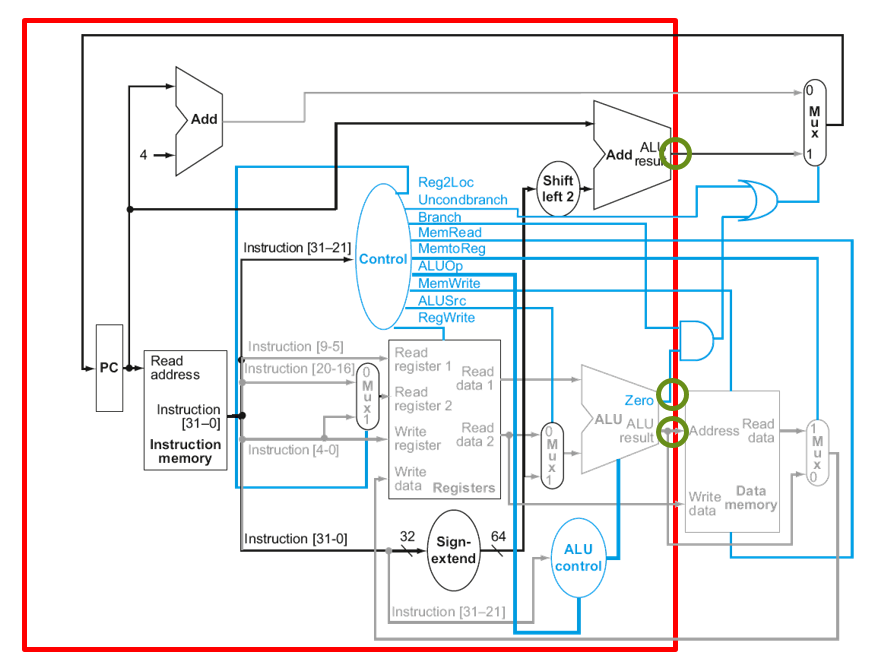
\includegraphics[width=4.75in]{../images/integrated_execute.png}
	\end{center}
\end{figure} 

\section{Your Assignment}

You are to:
\begin{enumerate}
\item Integrate your iExecute module into your datapath.v that includes iFetch and iExecute.
\item Update your Expected Results Table to include the new outputs.
\item Verify that your simulation results match your expected results.
\item Create a lab report in the LabN format that focuses on the integration of the iExecute stage.  The only inputs that you need to list are the inputs that you set in the initial section of datapath.v.  The only outputs are the signals that are leaving the red box in Figure ~\ref{fig:integrated_execute}. 
\end{enumerate}